\documentclass[autodetect-engine,dvipdfmx-if-dvi,ja=standard,everyparhook=compat]{bxjsarticle}

\usepackage{graphicx}        % 図を表示するのに必要
\usepackage{color}           % jpgなどを表示するのに必要
\usepackage{amsmath,amssymb} % 数学記号を出すのに必要
\usepackage{type1cm}         % fontsizeのエラー回避
\usepackage{here}            % 図の強制配置
\usepackage{url}             % URLをいい感じにしてくれる
\usepackage{subfigure}       % 図をまとめて表示
\usepackage{pdfpages}        % PDFの連結
\usepackage{setspace}
\usepackage{cases}
\usepackage{fancyhdr}
\usepackage{wrapfig}% 図の回り込み


% 余白の設定
% \setlength{\textheight}{\paperheight}   % 紙面縦幅を本文領域にする(BOTTOM=-TOP)
% \setlength{\topmargin}{-15.4truemm}     % 上の余白を10mm(=1inch-15.4mm)に
% \addtolength{\topmargin}{-\headheight}  %
% \addtolength{\topmargin}{-\headsep}     % ヘッダの分だけ本文領域を移動させる
% \addtolength{\textheight}{-20truemm}    % 下の余白も10mm
% \setlength{\textwidth}{\paperwidth}     % 紙面横幅を本文領域にする(RIGHT=-LEFT)
% \setlength{\oddsidemargin}{-5.4truemm}  % 奇数ページの左の余白を20mm(=1inch-5.4mm)に
% \setlength{\evensidemargin}{-5.4truemm} % 偶数数ページの左の余白を20mm(=1inch-5.4mm)に
% \addtolength{\textwidth}{-40truemm}     % 右の余白も20mm

% タイトル
\title{タイトル}

% ヘッダとフッタの設定
% \lhead{電気電子情報工学実験}
% \chead{}
% \rhead{20315784 佐藤凌雅}
% \lfoot{}
% \cfoot{\thepage} % ページ数
% \rfoot{}

\parindent = 0pt  % 行頭の字下げをしない
\setstretch{1.0}  % 行間

% キャプションの英語化
\renewcommand{\figurename}{Fig.}
\renewcommand{\tablename}{Table}

% 各章,節などタイトルの大きさを変更
% \titleformat*{\section}{\Huge\bfseries}
% \titleformat*{\subsection}{\Large\bfseries}

% 式の番号を(senction_num.num)のようにする
% \makeatletter
% \@addtoreset{equation}{chapter}
% \def\theequation{\thechapter.\arabic{equation}}
% \makeatother

% 呼び出したページのページ番号を消す
\newcommand{\deletePageNum}{
    \thispagestyle{empty}
    \clearpage
    \addtocounter{page}{-1}
}

% urlのフォントを直す
\renewcommand\UrlFont{\rmfamily}


\begin{document}
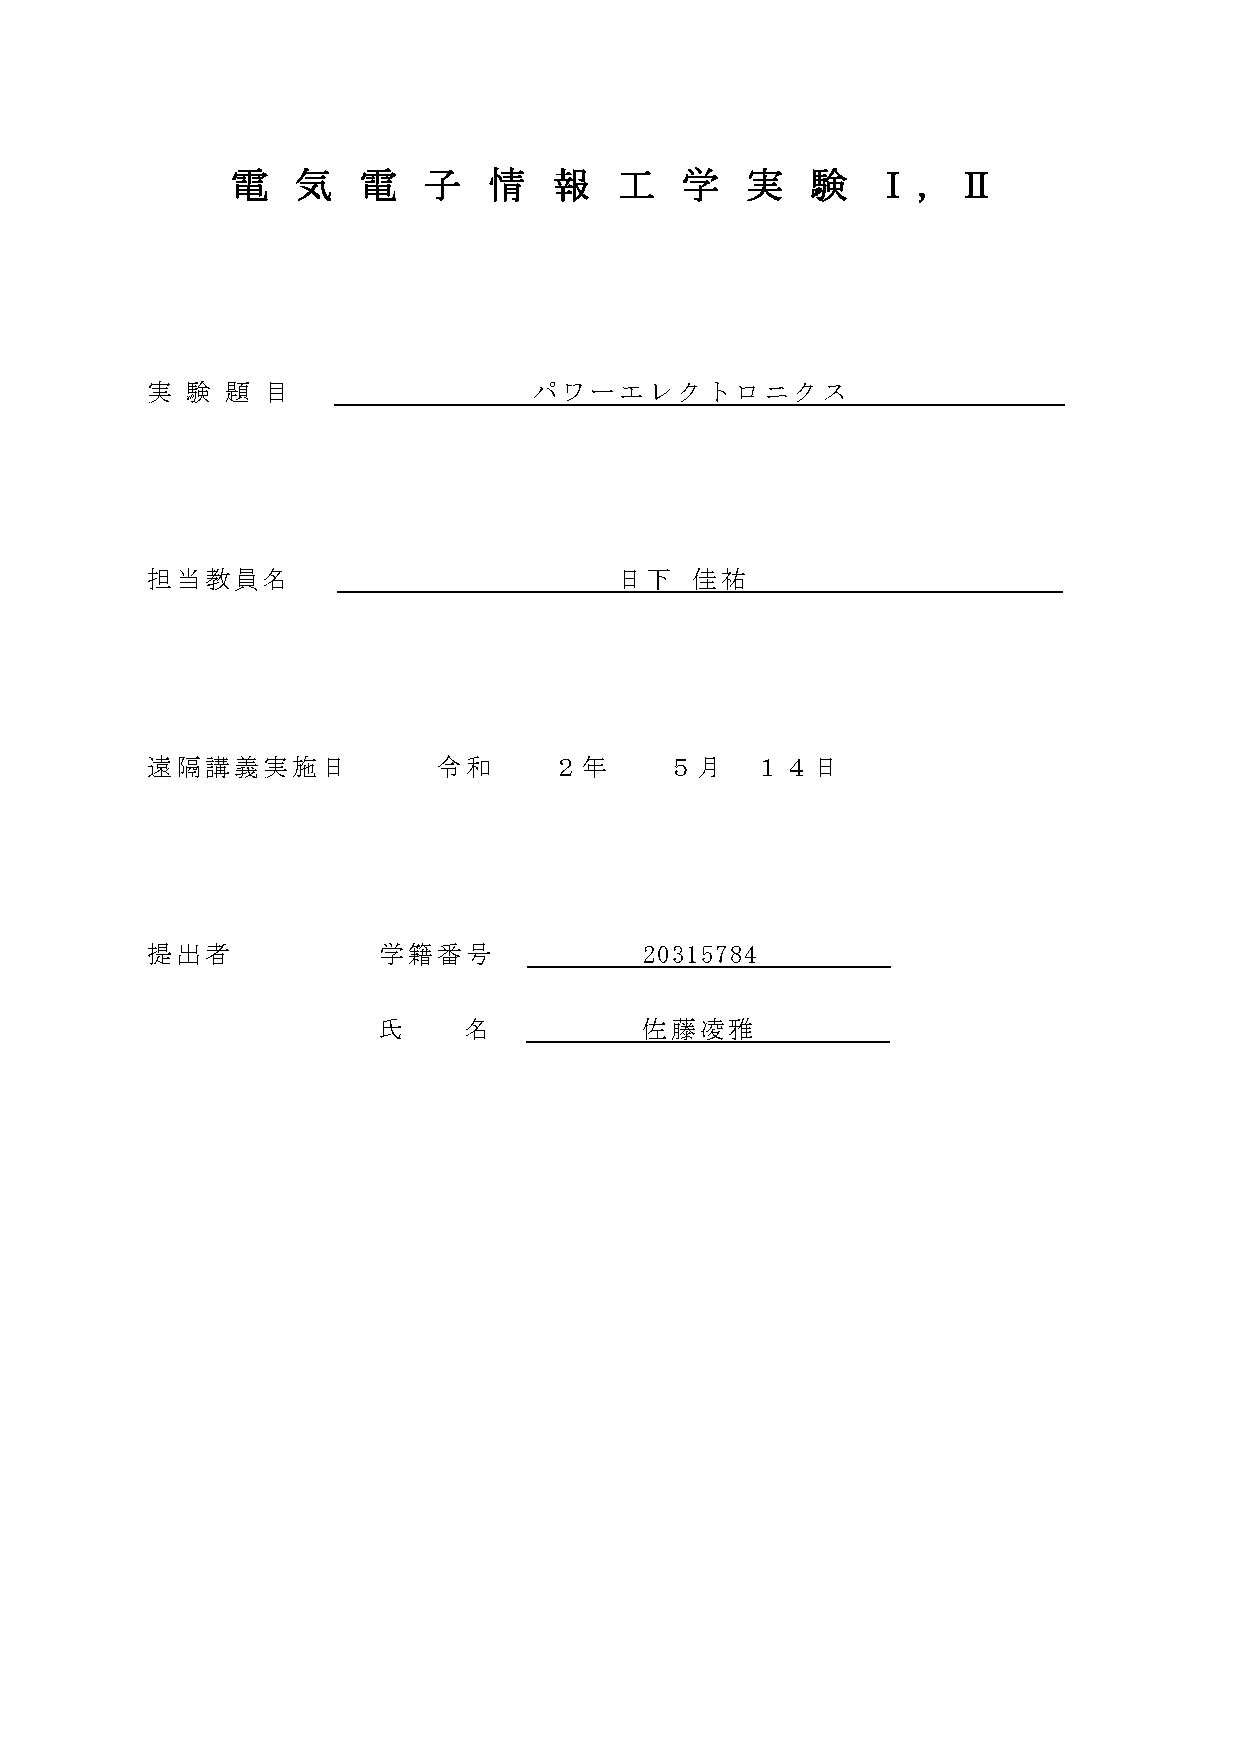
\includepdf[pages=-]{./setting/cover.pdf}
% \maketitle

\fontsize{11.041pt}{16.562pt}\selectfont

% 実験の目的,手段,結果,結論を簡潔にまとめ示すこと.(250字程度)
\section{概要 Abstract}
 この実験ではダイオード整流器,降圧チョッパ回路,インバータの動作原理を理解することを目的とする.ダイオード整流器においては回路パラメータの変化に対する入力電流,出力電圧の動作の違いについて,降圧チョッパ回路についてはデューティ $d$ と負荷抵抗 $R$ が回路動作に及ぼす影響を,インバータでは変調方式による動作の違いとモータ負荷による駆動特性を調査した.

% テキストに書かれている目的等を参考に,各自どの点に注目して実験したのかを明確に示すこと.(300字程度)
\section{目的 Purpose}
 実験を通じてダイオード整流器,降圧チョッパ回路,インバータの動作原理を理解することを目的とする.
\begin{enumerate}
    \item ダイオード整流器において, 回路パラメータ(平滑コンデンサ,負荷抵抗,リアクトル)の変化に対する入力電流,出力電圧の動作の違いについて調査,検討を行う.
    \item PWM駆動される降圧チョッパ回路において,デューティ $d$ と負荷抵抗 $R$ が回路動作(出力電圧,リアクトル電流)に及ぼす影響を調査,検討を行う.
    \item インバータの変調方式(PWM 4kHz,PWM 16kHz,方形波)による動作の違いを調査,検討する.
    \item インバータのモータ負荷による駆動特性を調査,検討する.
\end{enumerate}
 また,各種実験機器の使用方法,および注意事項についても同時に習得する.


% 各自の実験目的に必要な理論的な背景を示すこと.必要ならば,参考文献リストより文献番号を引用すること.(レポート用紙1枚程度)
\section{理論的背景 Theory}
\subsection{ダイオード整流器の動作原理}
\subsubsection{単相全波整流器$^{\cite{shinzui_single}}$}
 単相全波整流回路は,整流素子を用いた,交流電圧から直流電圧を得るための整流回路である.ダイオードを用いた単相全波整流回路の構成をFig.\ref{fig:single_phase_full_wave_rectifier_circuit}(a)に示す.この整流回路に対して入力として正弦波交流電圧 $v = \sqrt{2} V \sin \omega t$ を印加する場合を考える.この時の電流の流れる経路はFig.\ref{fig:single_phase_full_wave_rectifier_circuit}(b)に示すように2通りとなる.\\
 まず,入力電圧 $v$ が正のとき,ダイオード $D_1$ および $D_4$ の両端に順方向電圧がかかる.これらが導通することにより,電流の経路はFig.\ref{fig:single_phase_full_wave_rectifier_circuit}(b)の青線のようになる.また,負荷の両端には正の正弦波電圧が現れる.\\
 一方,交流電圧 $v$ が負のとき,ダイオード $D_2$ および $D_3$ の両端に順方向電圧がかかる.これらが導通することにより,電流の経路はFig.\ref{fig:single_phase_full_wave_rectifier_circuit}(b)の赤線のようになる.このとき,電流の流れる方向は $v$ が正のときと同じであり,負荷の両端には正の正弦波電圧が現れる.\\
 以上より,出力電圧 $e_d$ および電流 $i_d$の波形はFig.\ref{fig:single_phase_full_wave_rectifier_graph}のようになる.
\begin{figure}[H]
    \begin{center}
    \subfigure[Circuit]{%
        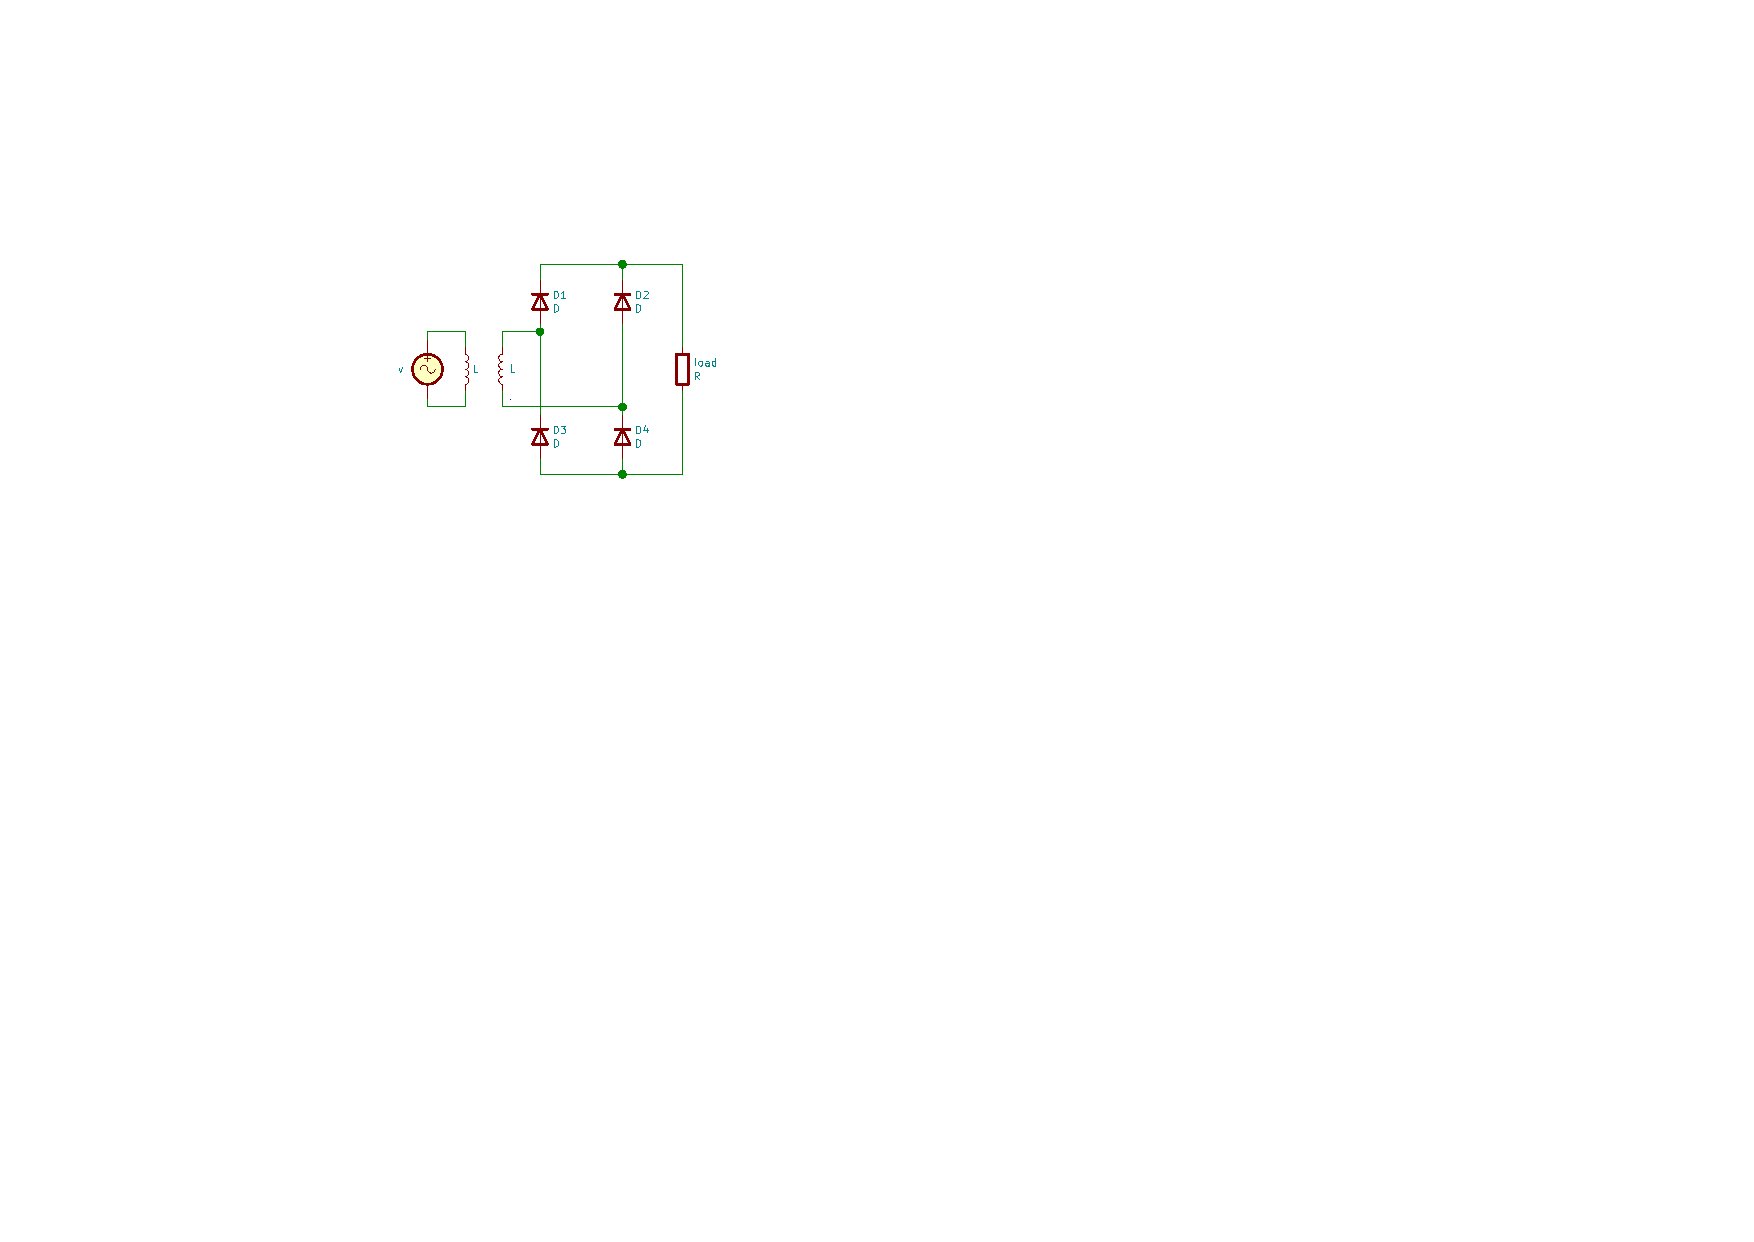
\includegraphics[clip, width=0.50\columnwidth]{./fig/single_phase_full_wave_rectifier_circuit.pdf}}%
    % \hspace{5truemm}
    \subfigure[Current path]{%
        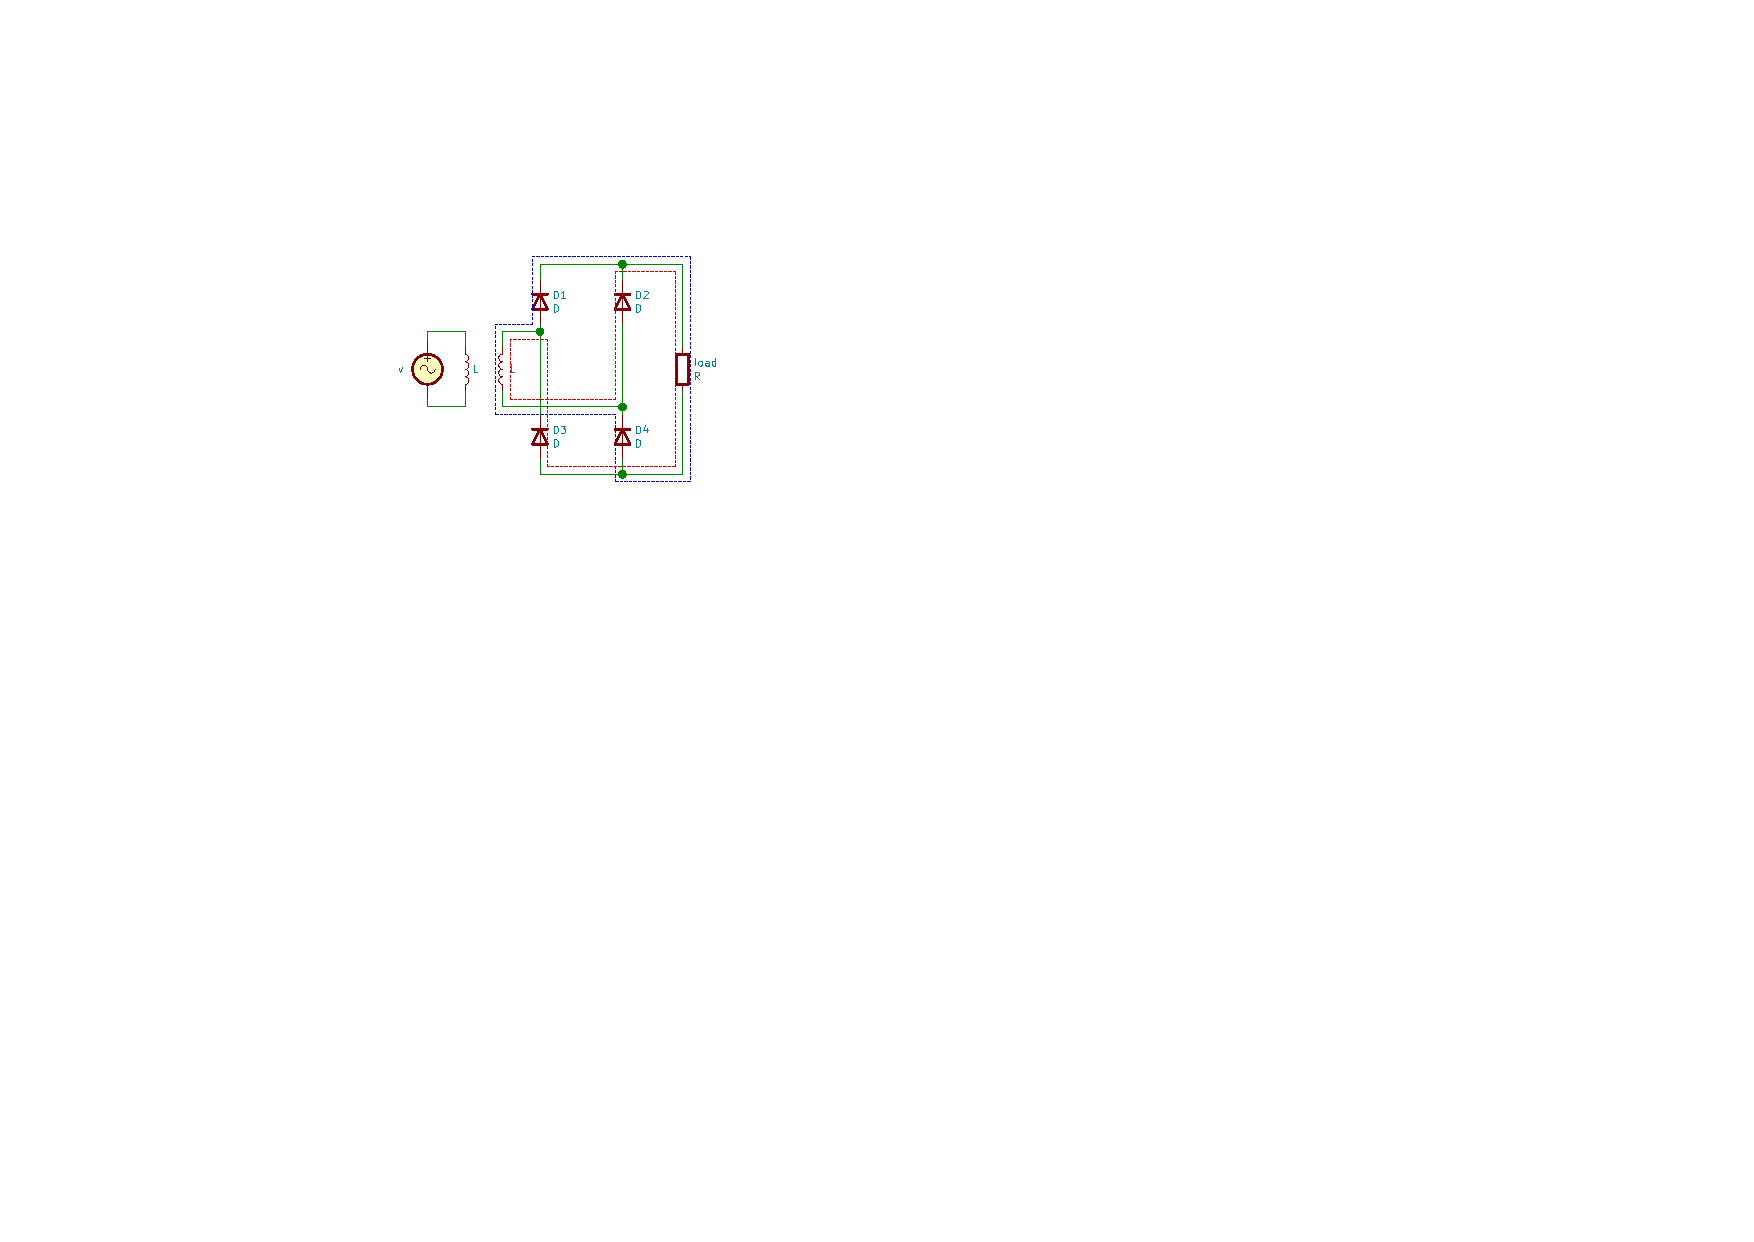
\includegraphics[clip, width=0.50\columnwidth]{./fig/single_phase_full_wave_rectifier_current_path.pdf}}%
    \end{center}
    \caption{Single-phase full-wave rectifier}
    \label{fig:single_phase_full_wave_rectifier_circuit}
\end{figure}

\begin{figure}[H]
    \centering
    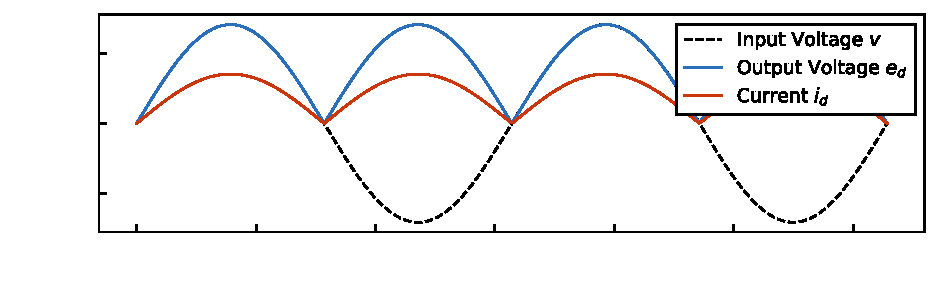
\includegraphics[width=15cm]{./fig/single_phase_full_wave_rectifier_graph.pdf}
    \caption{Voltage and current waveform of single-phase full-wave rectifier}
    \label{fig:single_phase_full_wave_rectifier_graph}
\end{figure}

\subsubsection{三相全波整流器$^{\cite{shinzui_three}}$}
 三相全波整流回路は,整流素子を用いた,交流電圧から直流電圧を得るための整流作用をもつ回路の一種で,三相の正弦波交流電圧のうち高低2つの相の差電圧を整流するのが特徴である.ダイオードを用いた単相全波整流回路をの構成をFig.\ref{fig:three_phase_full_wave_rectifier}(a)に示す.\\

 Fig.\ref{fig:three_phase_full_wave_rectifier}(a)のダイオードによる三相全波整流回路に純抵抗負荷を接続し,三相平衡電圧 $v_1$ 〜 $v_2$ を印加した場合の線間電圧 $v_{12}$ 〜 $v_{32}$ および出力電圧 $e_d$ の波形をFig.\ref{fig:three_phase_full_wave_rectifier}(b)に示す.\\

 上段のダイオード $D_1$ 〜 $D_3$ は最も電圧の高い相に接続しているものが導通し,上段のダイオード $D_4$ 〜 $D_6$ は最も電圧の低い相に接続しているものが導通するので,出力電圧 $e_d$ は線間電圧波形が整流された山なりの波形(Fig.\ref{fig:three_phase_full_wave_rectifier}(b)の黒色の波形)となる.
\begin{figure}[H]
    \begin{center}
    \subfigure[Circuit]{%
        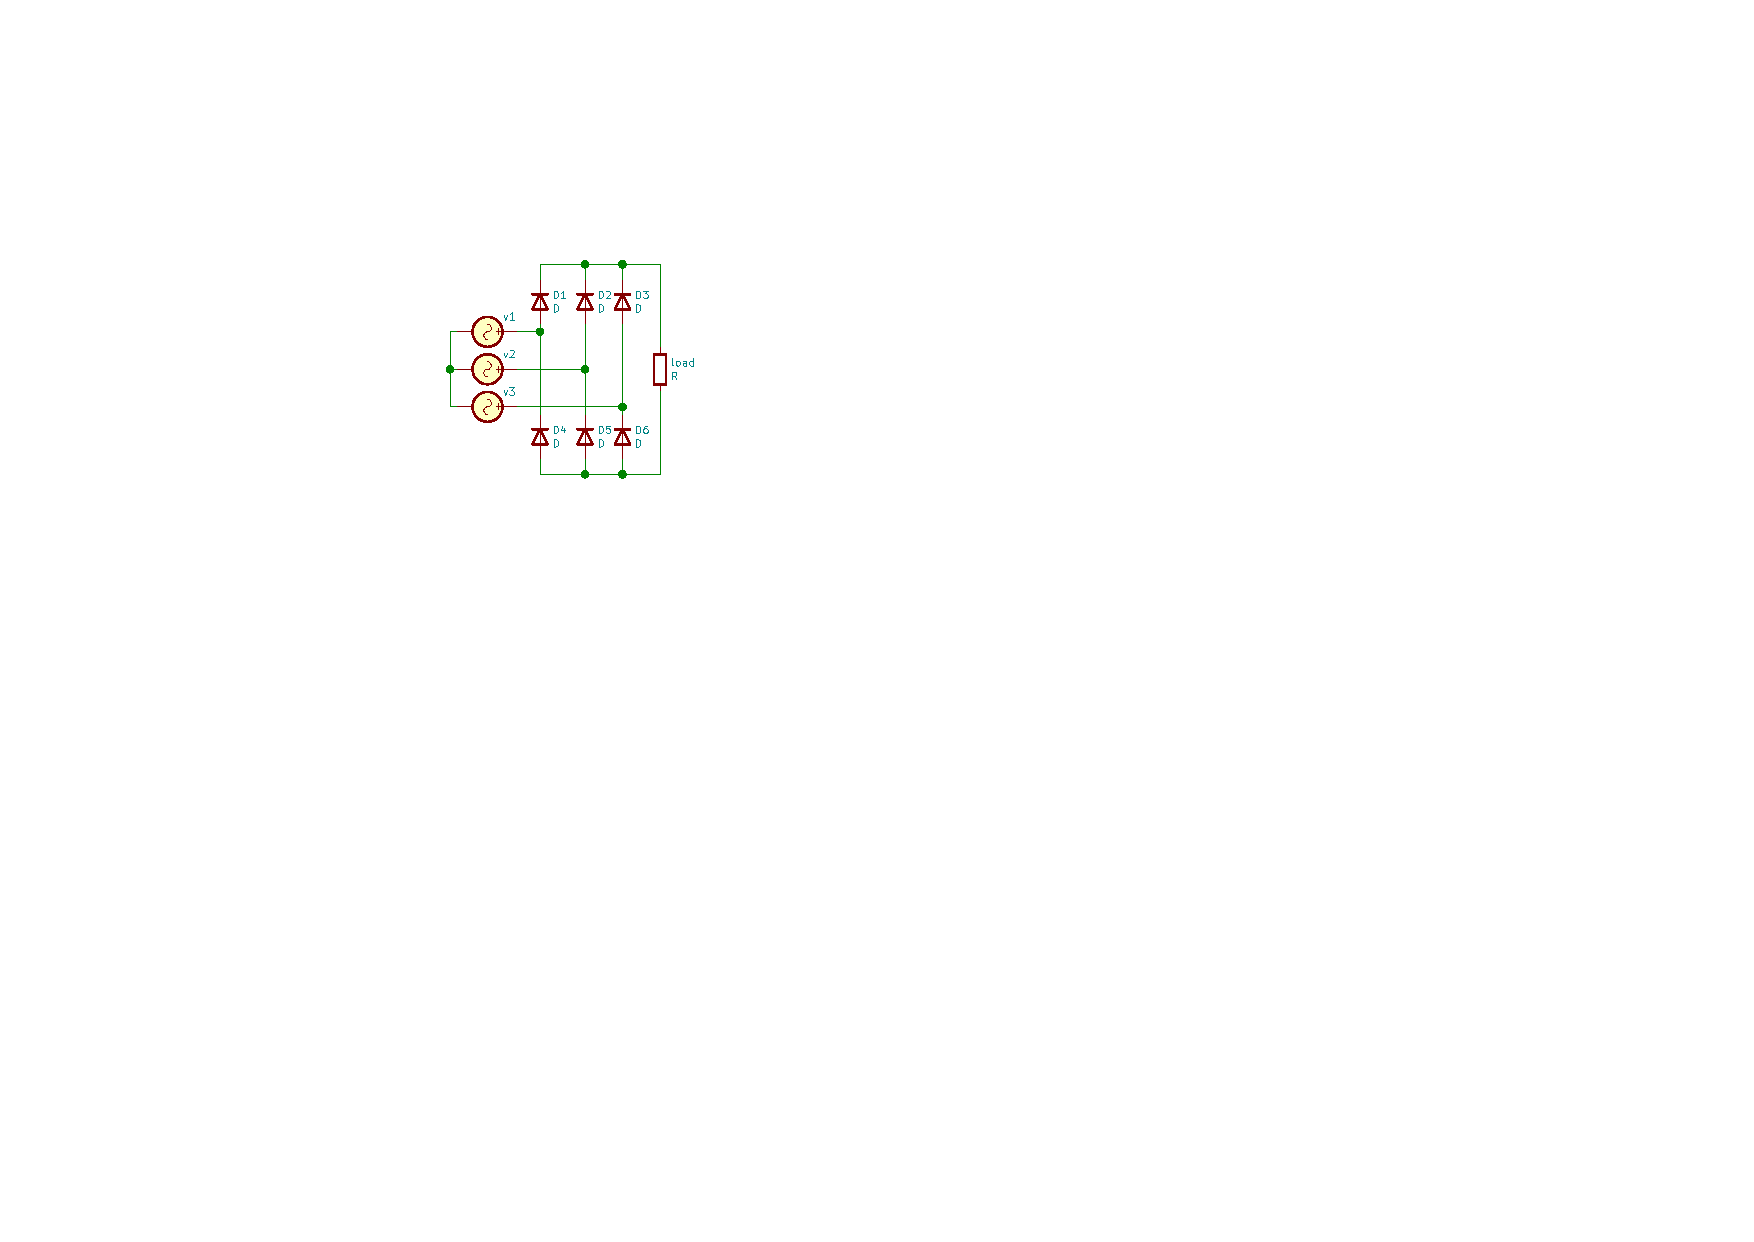
\includegraphics[clip, width=0.3\columnwidth]{./fig/three_phase_full_wave_rectifier_circuit.pdf}}%
    % \hspace{5truemm}
    \subfigure[Voltage and current waveform ]{%
        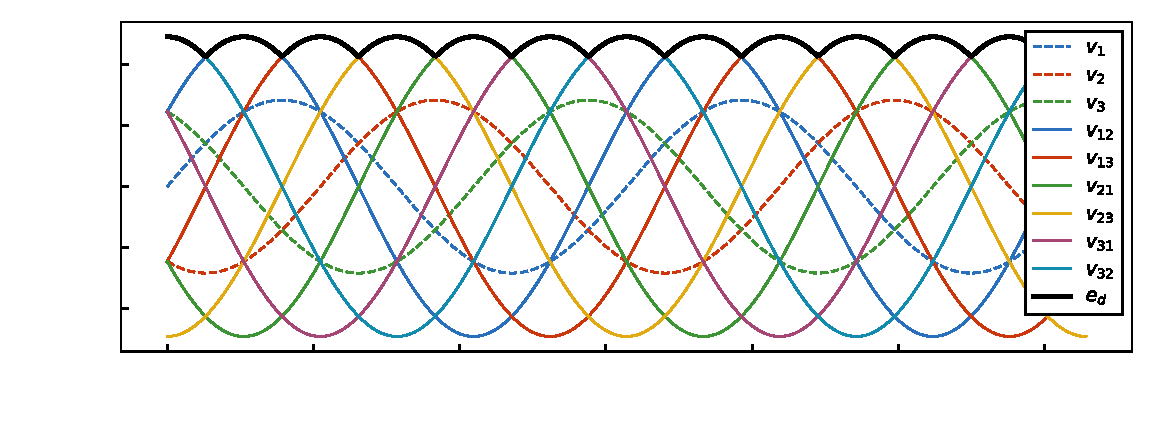
\includegraphics[clip, width=0.68\columnwidth]{./fig/three_phase_full_wave_rectifier_graph.pdf}}%
    \end{center}
    \caption{Three-phase full-wave rectifier}
    \label{fig:three_phase_full_wave_rectifier}
\end{figure}

\subsection{降圧チョッパ回路の動作原理$^{\cite{denkikigairon}}$}
 交流電力の電圧の大きさを効率よく昇降圧させるには変圧器を用いるが,直流電力の電圧調整には直流チョッパがよく用いられる.\\
 チョッパとは直流電圧を高頻度でオンオフ動作を行い,他の大きさの直流電圧に変換する回路をいう.Fig\ref{fig:chopper_circuit}にチョッパ回路の回路図を示す.

\begin{figure}[H]
    \centering
    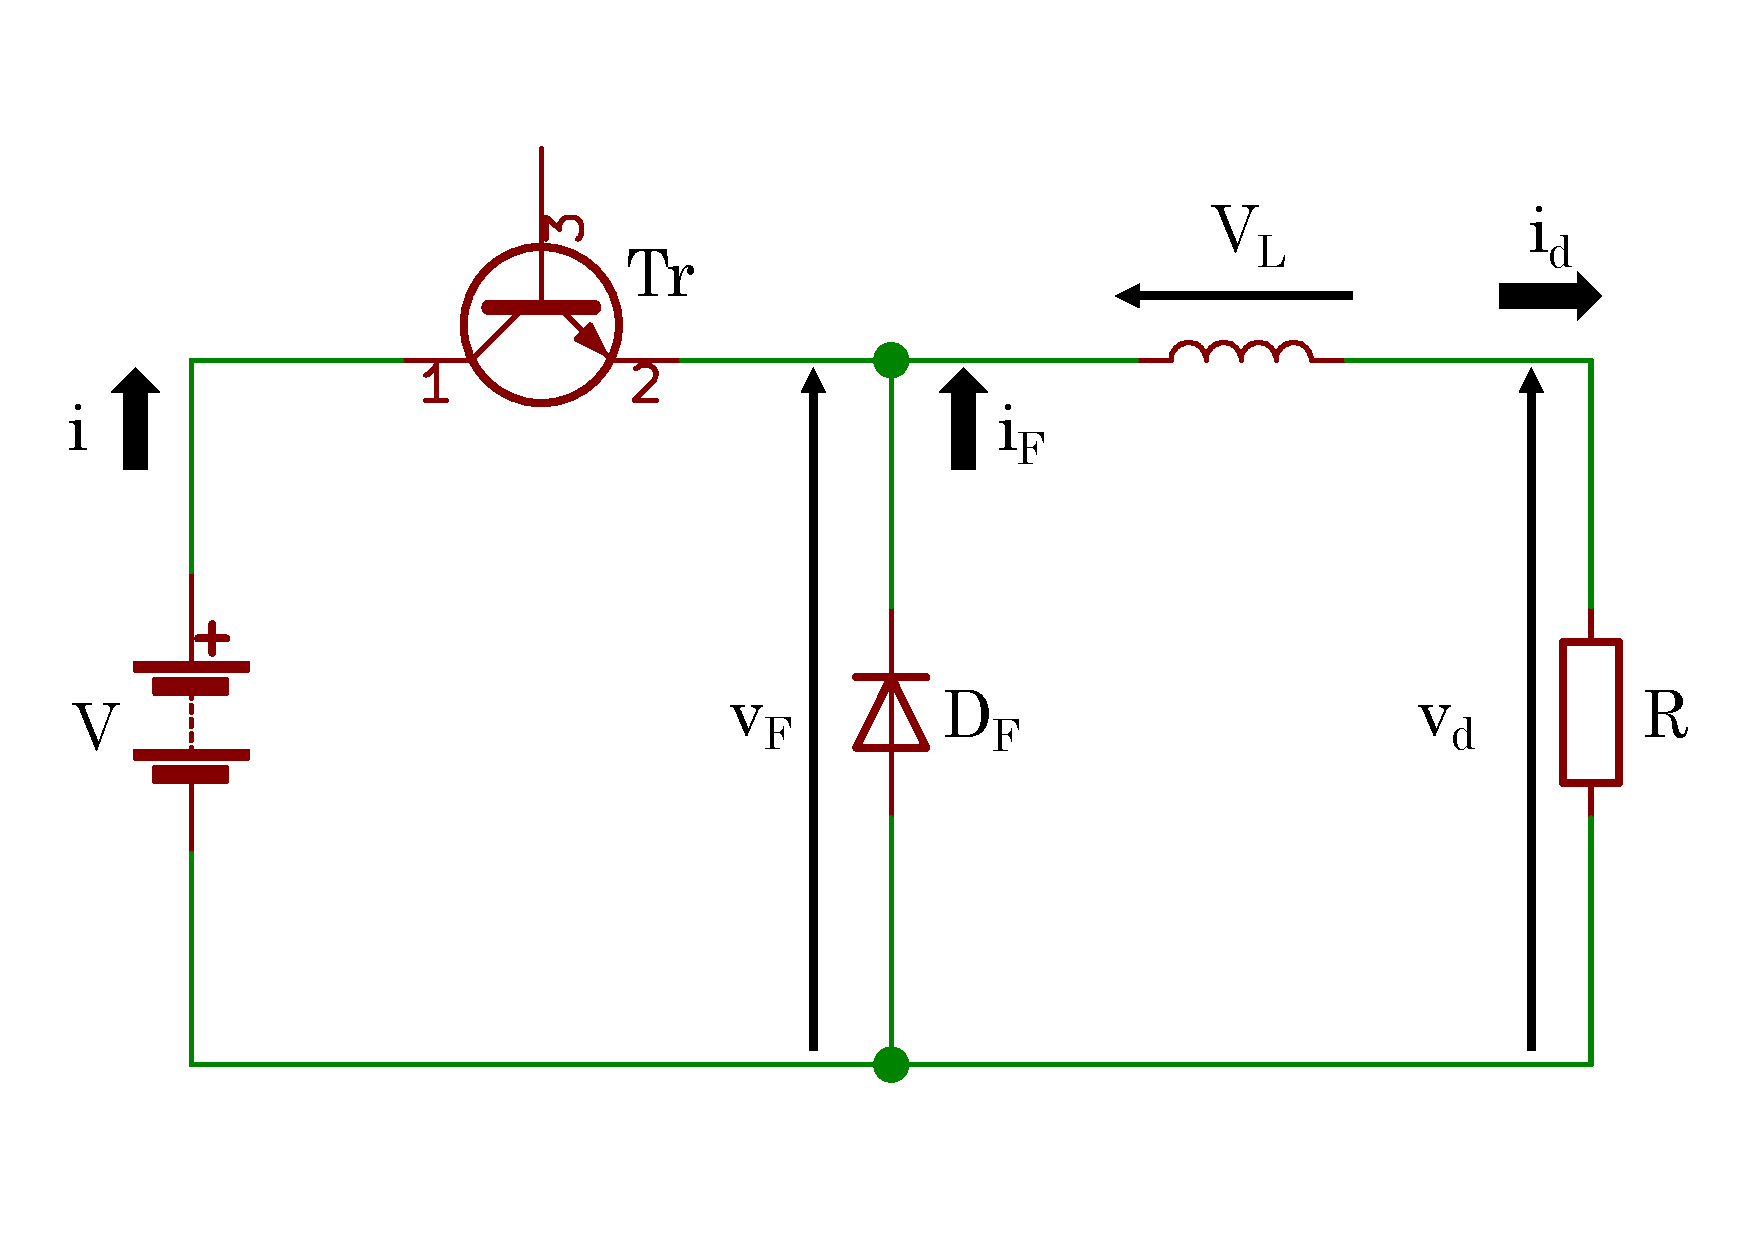
\includegraphics[width=8cm]{./fig/chopper_circuit.pdf}
    \caption{Chopper circuit}
    \label{fig:chopper_circuit}
\end{figure}

 チョッパ回路は以下の素子より構成されている
\begin{itemize}
    \item チョップ部 $T_r$:オンオフ動作を行うスイッチング素子(Tr,IGBT,MOSFETなど)
    \item リアクトリアル $L$[H]:負荷 $R$ に加わる電圧 $V_d$ や流れる電流 $i_d$ のリプルを小さくする
    \item 還流ダイオード $D_F$:チョップ部がオフの時の電流経路を構成する
\end{itemize}
 回路の動作は,チョップ部がオンの期間 $T_{ON}$[s] では,負荷には電源電流 $i$ が流れ,リアクトリアル $L$ には電圧 $v_L$ が生じる.次にチョップ部がオフの期間 $T_{OFF}$[s] では,リアクトリアル $L$ に蓄えられたエネルギーが電流 $i_L$ となって還流ダイオード $D_F$ を通り,負荷に還流する.このため,負荷電流 $i_d$ はFig.\ref{fig:chopper_current_graph}に示すような連続した脈動電流となる.\\

\begin{figure}[H]
    \centering
    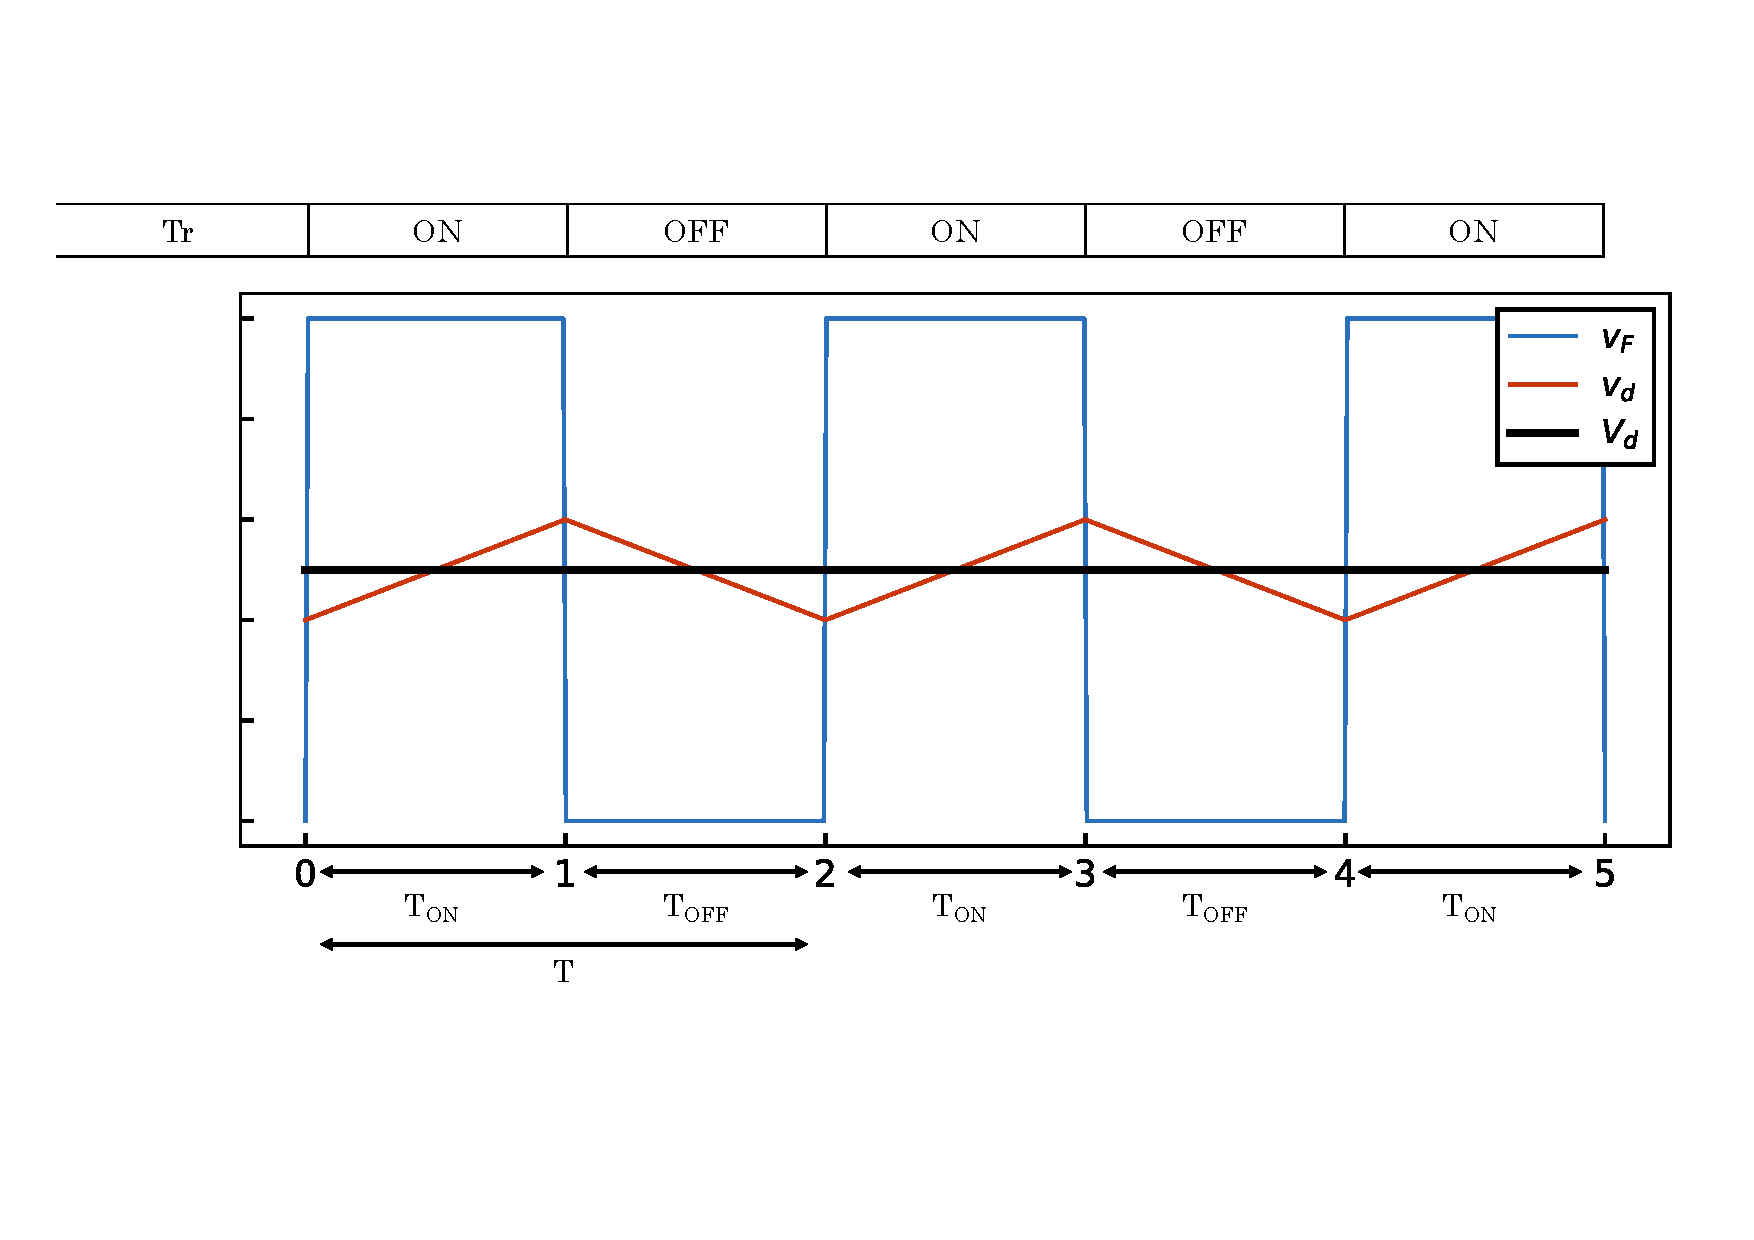
\includegraphics[width=12cm]{./fig/chopper_graph.pdf}
    \caption{Voltage graph of the chopper circuit}
    \label{fig:chopper_graph}
\end{figure}

\begin{figure}[H]
    \centering
    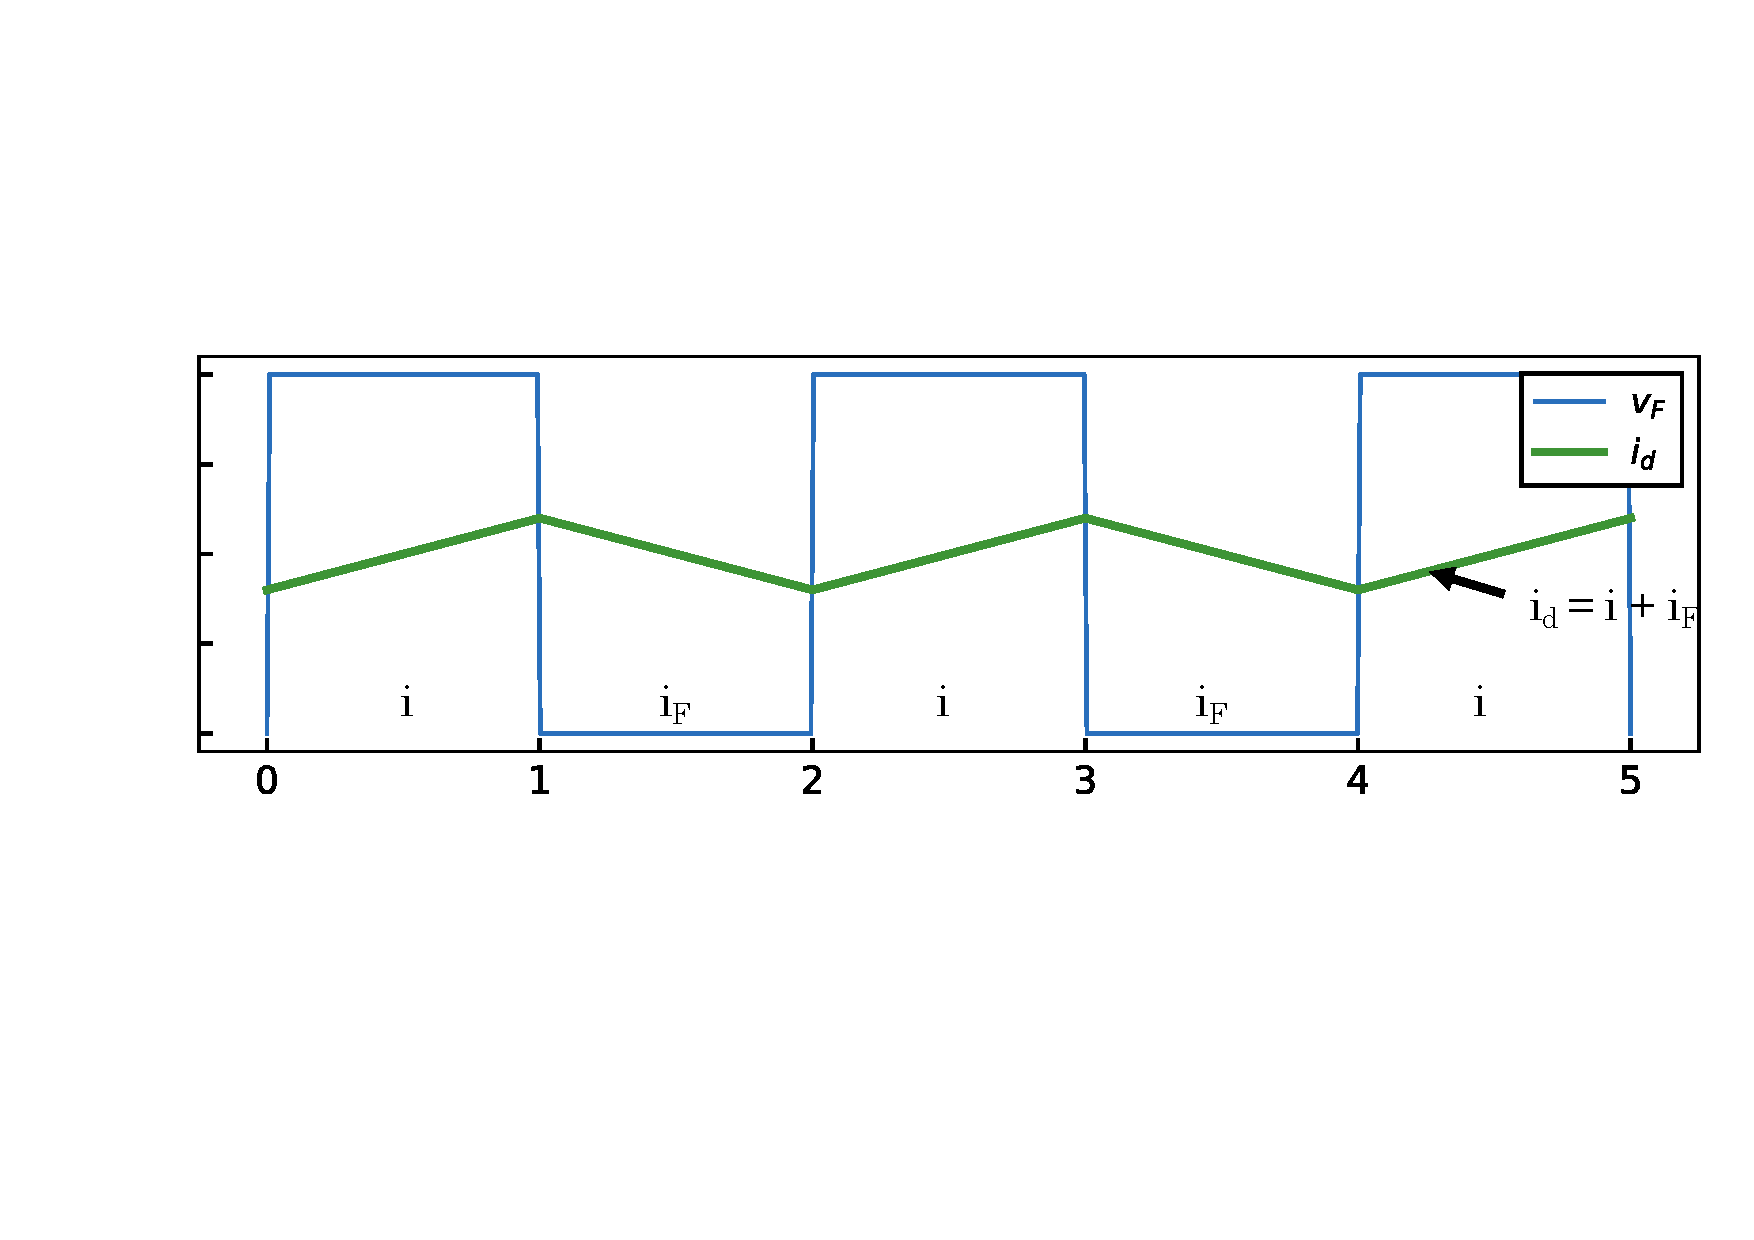
\includegraphics[width=12cm]{./fig/chopper_current_graph.pdf}
    \caption{Current graph of a chopper circuit}
    \label{fig:chopper_current_graph}
\end{figure}

 なお,負荷電圧 $v_d$ はチョップ部がオンの時,電源電圧 $V$ と リアクトリアル $L$ に生じる電圧 $v_L$ との差となる.チョップ部がオフ時にはリアクトリアル $L$ に蓄えられたエネルギーが放出電流 $i_F$ として抵抗 $R$ に流れ,負荷電圧 $v_d$ が生じる.\\
 この時,周期 $T$ でオンオフ動作を繰り返す時の出力電圧 $v_d$[V] の平均値,すなわち平均出力電圧 $V_d$[V] は以下の式で表される.
\begin{equation}
    V_d = \frac{T_{ON}}{T}V = \alpha V
    \label{eqn:average_output_voltage_of_the_chopper}
\end{equation}

 Eqn.(\ref{eqn:average_output_voltage_of_the_chopper})において $\frac{T_{ON}}{T}$ は1よりい小さいため,平均出力電圧 $V_d$ は電源電圧 $V$ より小さくなる.なお,オン期間 $T_{ON}$ の周期 $T$ に対する比 $\alpha$ を通流率という.

\subsection{インバータの動作原理$^{\cite{denkikigairon}}$}
 インバータは直流を交流に変換する装置である.Fig.\ref{fig:principle_of_the_inverter}にインバータの原理図を示す.
Fig.\ref{fig:principle_of_the_inverter}(a)において, $t_0$[s] で $S_1$ と $S_4$ を閉じると,負荷 $R$[$\Omega$] には左側が+極となる電源電圧 $V$[V] が加わり, $S_1$ → $R$ → $S_4$ へと負荷電流が流れる.\\
 次に $t_1$[s] で $S_1$ と $S_4$ を開くと同時に,$S_2$ と $S_3$ を閉じると,今度は右側が+極となる電源電圧 $V$[V] が負荷 $R$ に加わり,負荷電流は, $S_3$ → $R$ → $S_2$ へと流れる.再び, $t_2$[s] で $S_2$ と $S_3$ を開くと同時に,$S_1$ と $S_4$ を閉じると, $t_0$[s] における状態に戻る.\\
 これを繰り返すと負荷 $R$ にはFig.\ref{fig:principle_of_the_inverter}(b)のような方形波状の交流電圧 $v_o$ が加わって,直流を交流に変換することができる.$t_0$ から $t_2$ までの時間 $T$[s] が1周期となり,この $T$ を変えることで,交流出力の周波数 $f$[Hz] を変えることができる.

\begin{figure}[H]
    \begin{center}
    \subfigure[Circuit]{%
        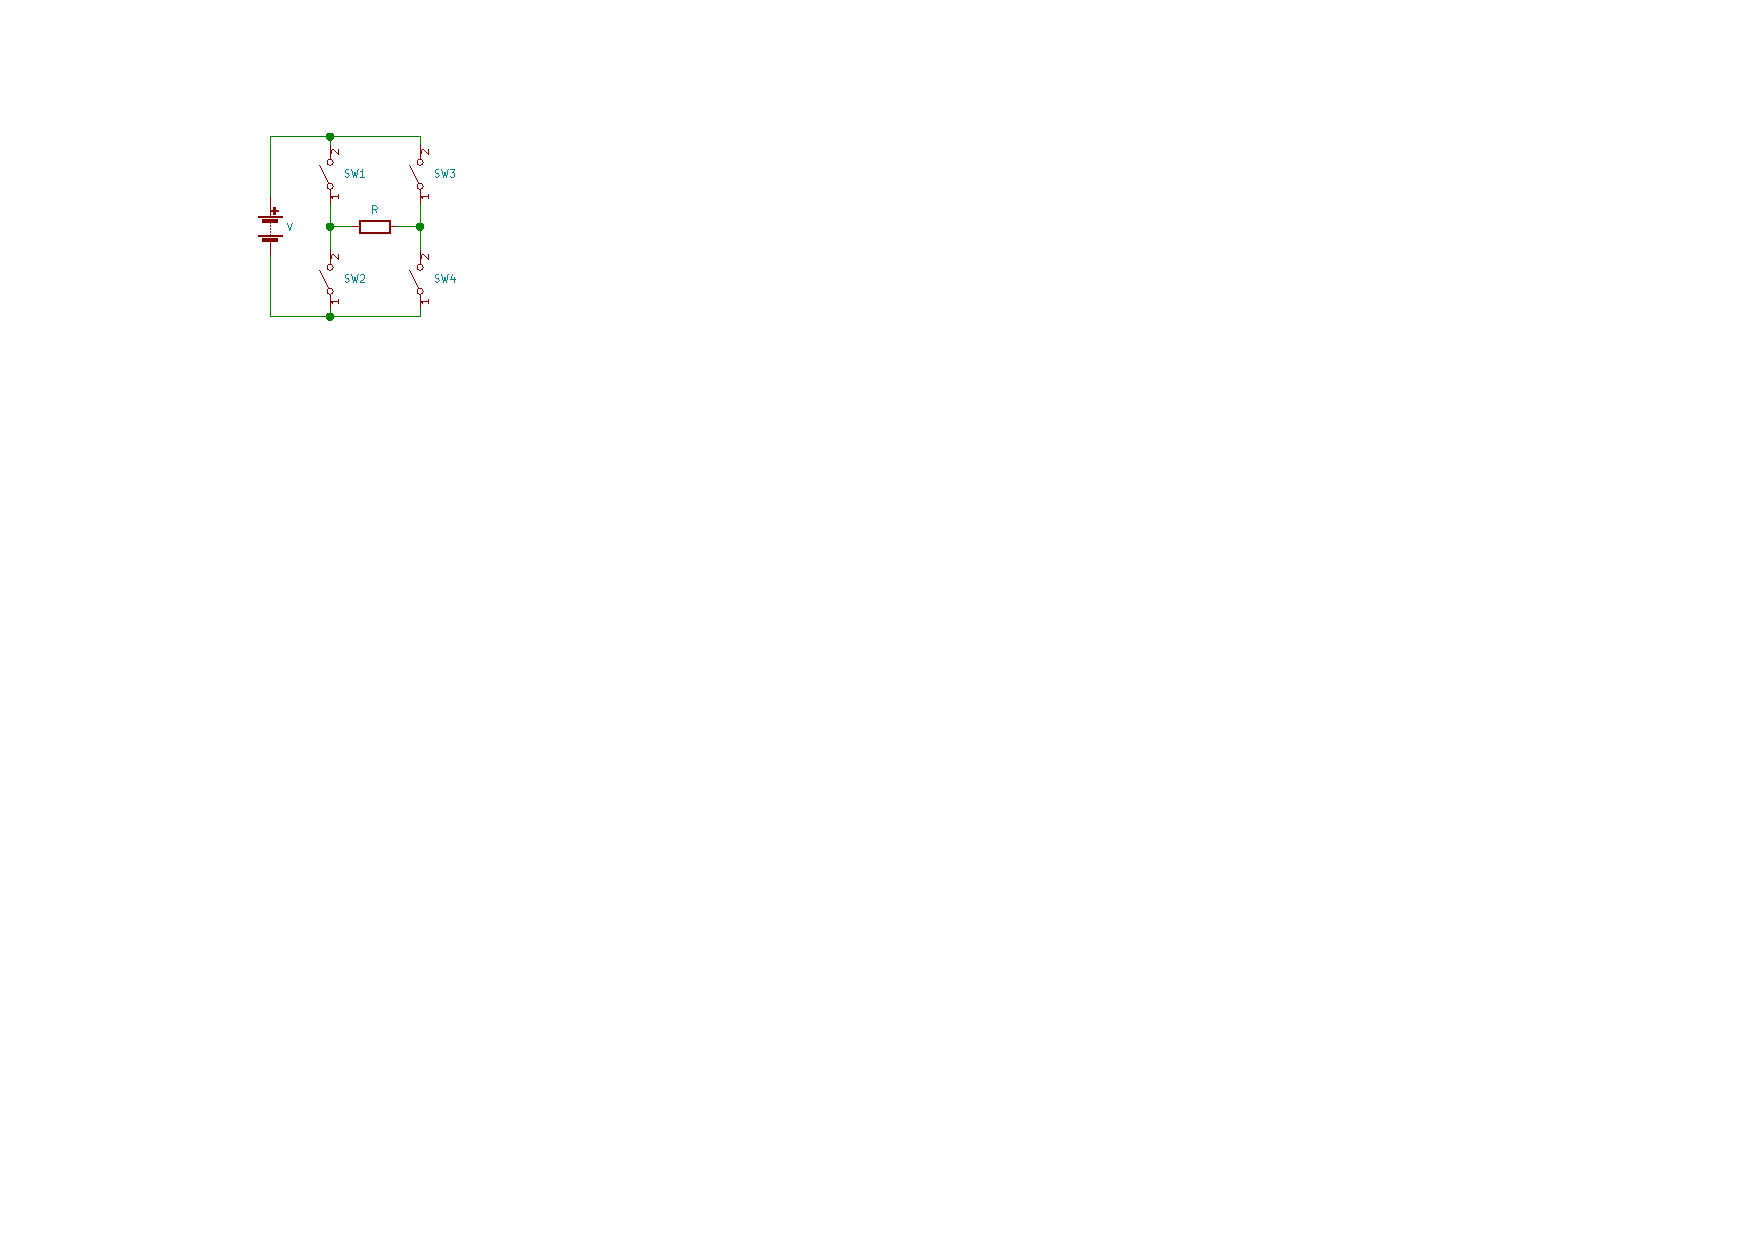
\includegraphics[clip, width=0.25\columnwidth]{./fig/inverter_circuit.pdf}}%
    \hspace{5truemm}
    \subfigure[Output voltage waveform]{%
        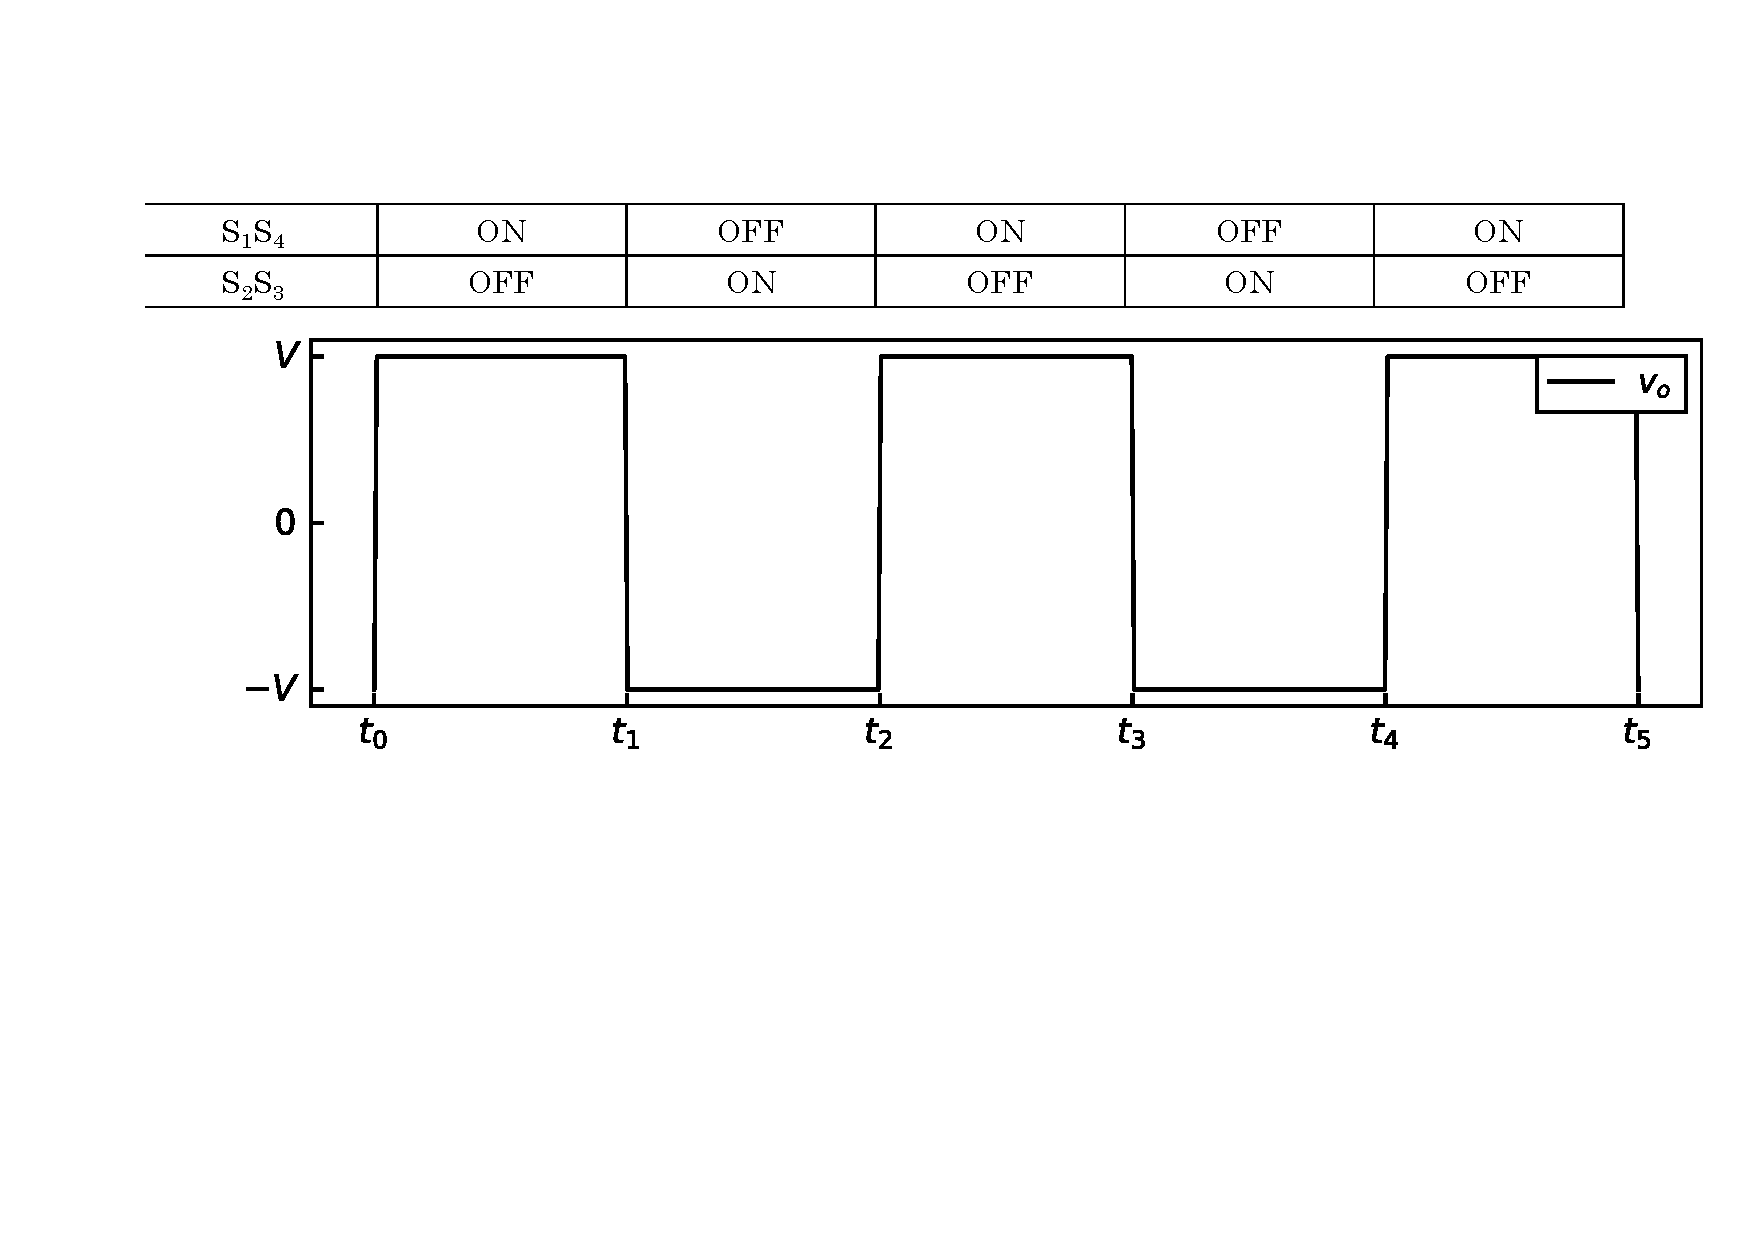
\includegraphics[clip, width=0.70\columnwidth]{./fig/inverter_graph.pdf}}%
    \end{center}
    \caption{Principle of the inverter}
    \label{fig:principle_of_the_inverter}
\end{figure}

 ここで,PWM駆動という駆動方法がある.PWMとはPulse Width Modulation(パルス幅変調)の略で,前述した方形波パルスをさらに分割し,パルス幅を時間的に変化させて高調波成分を減らすことが可能となる.\\
 PWM制御のうち,負荷が誘導性という条件のもとで,通電率を正弦波状に変化させれば出力電圧のパルス幅は正弦波の振幅に対応して変化し,出力電流波形は正弦波に近づく.\\
 PWM波形は,信号波(正弦波)と搬送波(三角波)をコンパレータに入力することで得られる.Fig.\ref{fig:PWM_graph}にPWMインバータの動作波形を示す.
\begin{figure}[H]
    \centering
    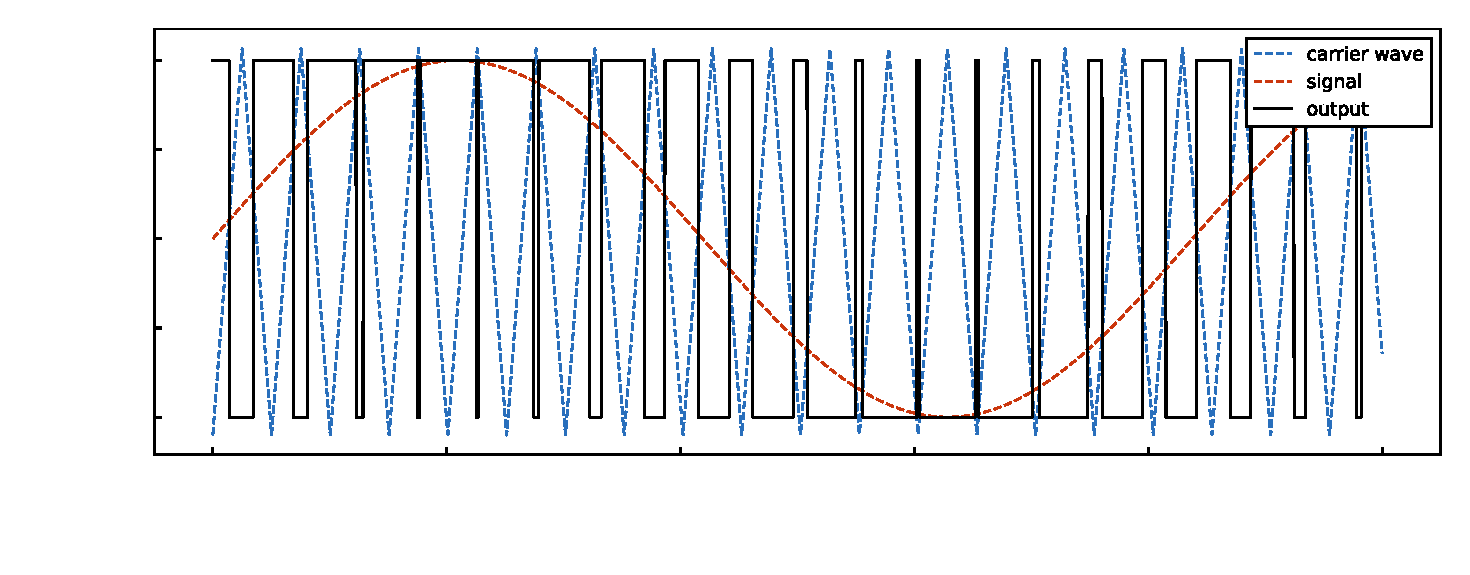
\includegraphics[width=15cm]{./fig/PWM_graph.pdf}
    \caption{PWM inverter operation waveform}
    \label{fig:PWM_graph}
\end{figure}


% 実験手段,測定系の概要,測定装置の名称・型番等を書くこと.また,装置の精度・仕様等の情報もできる限り示すこと.(レポート用紙2枚程度)
\section{実験方法 Experiment}

% 各自の実験目的に沿った結果を簡潔にまとめること.その他の試行錯誤的実験データは Appendix にまとめる.枚数は各教員の指示に従ってください.(レポート用紙の枚数は教員の指示に従う)
\section{実験結果 Results}

% 各自の目的と照らし合わせ,測定結果の妥当性や数値計算結果との整合性などについて考察する.実験結果とサブテキスト/参考書の図式とを比較し議論すること.課題が与えられているテーマに関してはそれについても考察すること.(レポート用紙2枚程度)
\section{考察 Discussion}

% 君自身が実験を通じて(実験の方法,まとめ方などで)工夫した点をまとめる.(100字程度 )
\section{工夫した点}

% 実験結果の羅列ではなく,考察した結果をまとめること.(250字程度)
\section{結論 Conclusion}

% レポートで引用した参考文献のリストを付ける.
\section{参考文献 Reference}
\begin{thebibliography}{9}
    \bibitem{shinzui_single} 電気の神髄. 単相全波整流回路(単相ブリッジ整流回路). \url{https://denki-no-shinzui.com/12544/}, (参照:2020-05-16)
    \bibitem{shinzui_three} 電気の神髄. 三相全波整流回路(三相ブリッジ整流回路). \url{https://denki-no-shinzui.com/12978/}, (参照:2020-05-16)
    \bibitem{denkikigairon} 深尾正 (2015). 電気機器概論. 実教出版株式会社.
\end{thebibliography}


% 周辺の関連調査事項,作成プログラムリスト,試行錯誤的実験データ
\appendix
\section{Appendix}

\end{document}
